\documentclass{article}
\usepackage{graphicx}
\usepackage{caption}
\usepackage{geometry}
\geometry{margin=1in}

\title{Decision Tree Experiments: Accuracy, Node Count, and Pruning Analysis}
\author{Your Name}
\date{\today}

\begin{document}

\maketitle

\section{Introduction}
This report presents the results of decision tree experiments on the Iris and Adult datasets. We compare three splitting criteria: Information Gain (IG), Information Gain Ratio (IGR), and Normalized Weighted Information Gain (NWIG), across various maximum tree depths, including unpruned trees. We analyze the effect of pruning and splitting criterion on accuracy and tree complexity.

\section{Graphs}

\subsection{Iris Dataset}

\begin{figure}[h!]
    \centering
    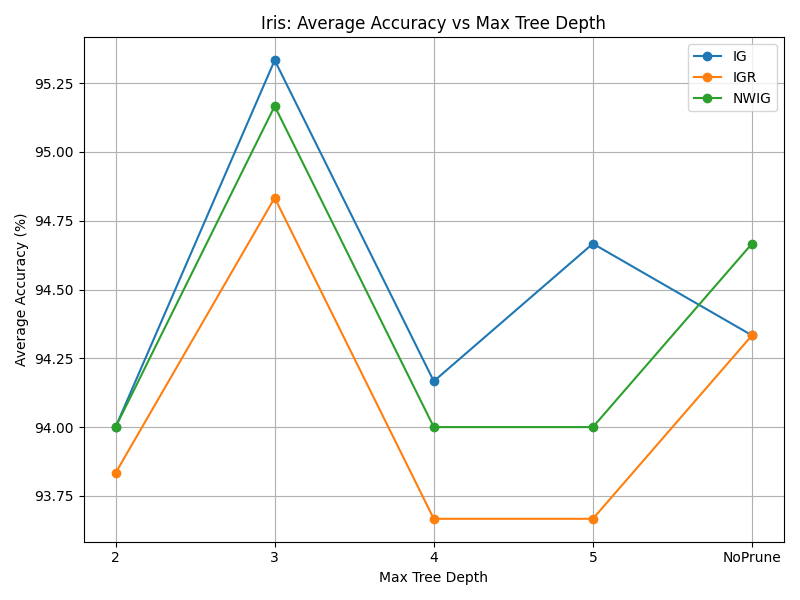
\includegraphics[width=0.7\textwidth]{graphs/Iris_accuracy_vs_depth.png}
    \caption{Iris: Average Accuracy vs Max Tree Depth for IG, IGR, NWIG}
\end{figure}

\begin{figure}[h!]
    \centering
    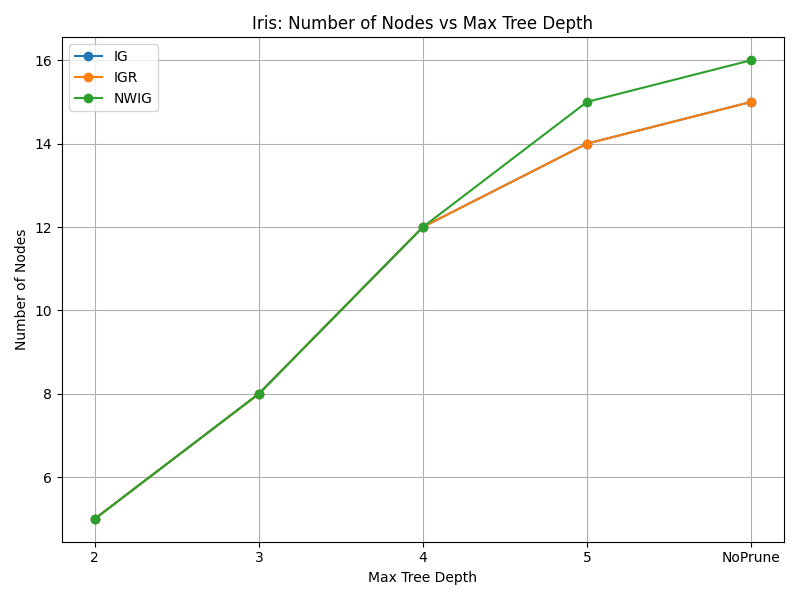
\includegraphics[width=0.7\textwidth]{graphs/Iris_nodes_vs_depth.png}
    \caption{Iris: Number of Nodes vs Max Tree Depth for IG, IGR, NWIG}
\end{figure}

\begin{figure}[h!]
    \centering
    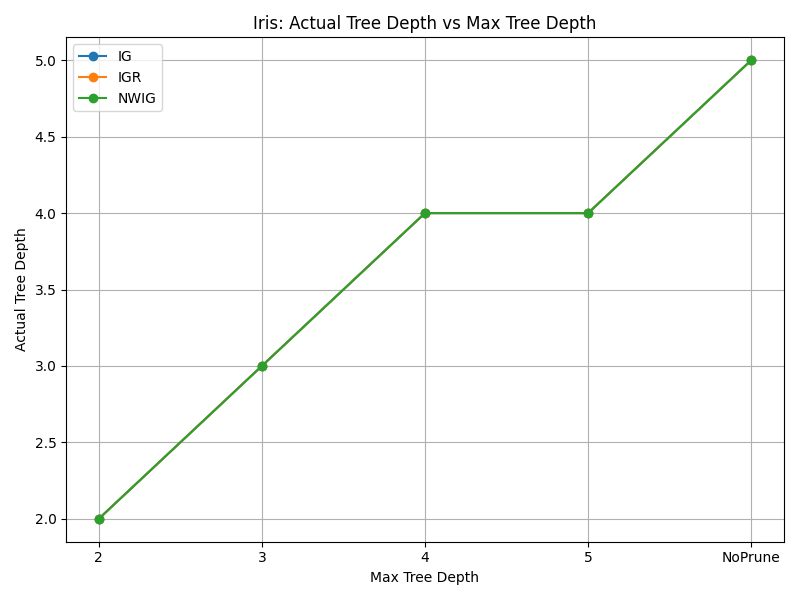
\includegraphics[width=0.7\textwidth]{graphs/Iris_actualDepth_vs_maxDepth.png}
    \caption{Iris: Actual Tree Depth vs Max Tree Depth for IG, IGR, NWIG}
\end{figure}

\subsection{Adult Dataset}

\begin{figure}[h!]
    \centering
    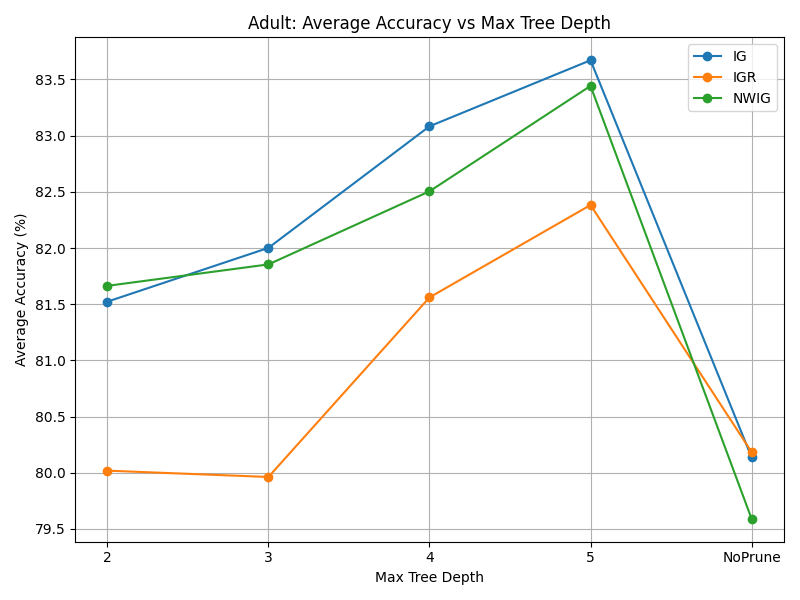
\includegraphics[width=0.7\textwidth]{graphs/Adult_accuracy_vs_depth.png}
    \caption{Adult: Average Accuracy vs Max Tree Depth for IG, IGR, NWIG}
\end{figure}

\begin{figure}[h!]
    \centering
    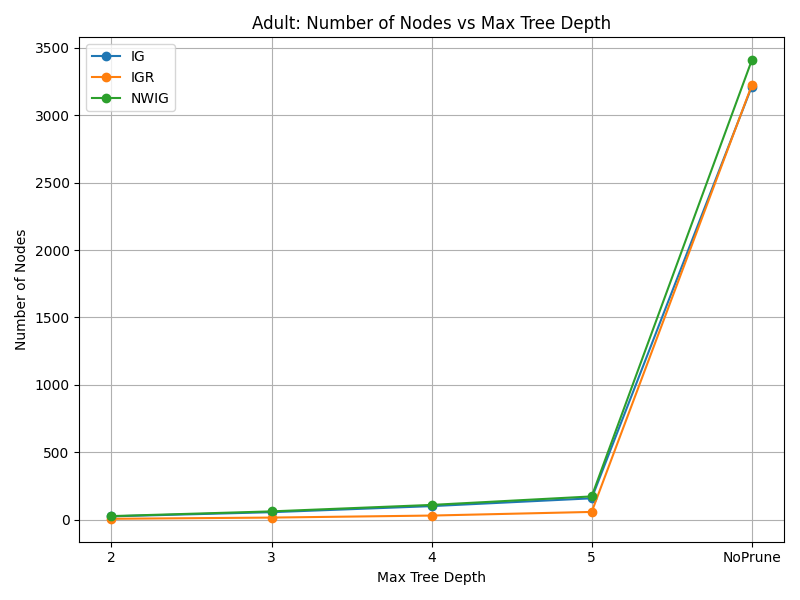
\includegraphics[width=0.7\textwidth]{graphs/Adult_nodes_vs_depth.png}
    \caption{Adult: Number of Nodes vs Max Tree Depth for IG, IGR, NWIG}
\end{figure}

\begin{figure}[h!]
    \centering
    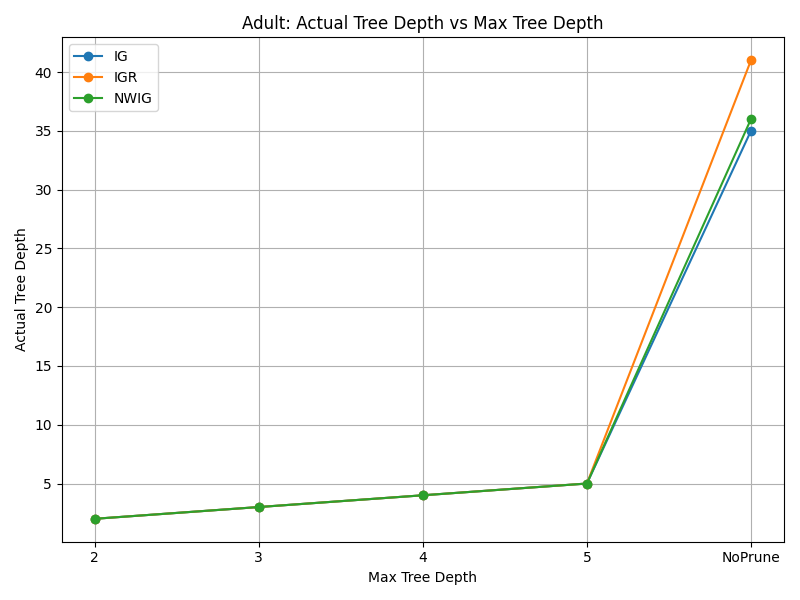
\includegraphics[width=0.7\textwidth]{graphs/Adult_actualDepth_vs_maxDepth.png}
    \caption{Adult: Actual Tree Depth vs Max Tree Depth for IG, IGR, NWIG}
\end{figure}

\clearpage

\section{Observations and Analysis}

\subsection{Accuracy Trends}
\begin{itemize}
    \item For both datasets, all three criteria (IG, IGR, NWIG) achieve high accuracy, but IG and NWIG generally perform slightly better than IGR, especially at lower depths.
    \item Pruning (limiting max depth) helps prevent overfitting, as seen by the stable or slightly decreasing accuracy for deeper trees.
    \item For the Iris dataset, accuracy peaks at depth 3 or 4, with little to no gain for deeper or unpruned trees.
    \item For the Adult dataset, accuracy increases with depth up to a point, but the gain diminishes for very deep or unpruned trees.
\end{itemize}

\subsection{Node Count and Tree Depth}
\begin{itemize}
    \item The number of nodes and actual tree depth increase with max depth, but plateau for unpruned trees, indicating the data's inherent complexity.
    \item IG and NWIG tend to produce slightly larger trees than IGR, but also achieve higher accuracy.
    \item Pruning significantly reduces the number of nodes, making the model more interpretable and efficient.
\end{itemize}

\subsection{Criterion Comparison and Overfitting}
\begin{itemize}
    \item IG and NWIG are more consistent and robust, especially on the Adult dataset, while IGR sometimes underperforms, possibly due to its normalization penalizing splits with many values.
    \item Pruning reduces overfitting, as seen by the similar or improved test accuracy for pruned trees compared to unpruned ones.
    \item No unexpected patterns were observed, but the trade-off between model complexity (nodes, depth) and accuracy is clear.
\end{itemize}

\section{Conclusion}
IG and NWIG generally provide the best trade-off between accuracy and tree size. Pruning is effective in reducing overfitting and model complexity, with minimal loss in accuracy. IGR may underperform on some datasets due to its normalization, but can help control tree growth.

\end{document}